\documentclass[UTF8,a4paper,11pt]{ctexart}

\usepackage[margin=2.35cm]{geometry}
\usepackage{amsmath,amssymb}
\usepackage{booktabs}
\usepackage{graphicx}
\usepackage{longtable}
\usepackage{array}
\usepackage{enumitem}
\usepackage{xcolor}
\usepackage{hyperref}
\usepackage{caption}
\usepackage{subcaption}
\usepackage{float}
\usepackage{fancyhdr}

\hypersetup{
  colorlinks=true,
  linkcolor=blue!55!black,
  urlcolor=blue!55!black,
  citecolor=blue!55!black
}
\graphicspath{{../}}
\setlist{nosep,leftmargin=2em}
\renewcommand{\arraystretch}{1.18}
\pagestyle{fancy}
\fancyhf{}
\setlength{\headheight}{14pt}
\fancyhead[L]{深度学习基础大作业报告}
\fancyhead[R]{股票趋势预测与模拟交易}
\fancyfoot[C]{\thepage}

\newcommand{\todo}[1]{\textcolor{red!70!black}{【待补充：#1】}}
\newcommand{\placeholderbox}[2]{
  \begin{center}
    \fbox{\parbox[c][#1][c]{0.9\linewidth}{\centering #2}}
  \end{center}
}

\title{\textbf{基于深度学习的 A 股短期收益预测与模拟交易}\\
  \large 深度学习基础课程大作业实验报告}
\author{
  组员 1：\todo{姓名、学号}\qquad
  组员 2：\todo{姓名、学号}\\[0.4em]
  分工：\todo{写明两位组员在数据、模型、回测、交易、报告中的具体工作}
}
\date{\today}

\begin{document}
\maketitle

\begin{abstract}
本文面向课程给定的 A 股日频量价数据，构建了从数据清洗、特征工程、标签定义、深度学习建模、历史回测到比赛交易辅助的完整流程。
项目使用 20 个横截面与时间序列特征，比较 MLP、LSTM 与 DLinear 三类神经网络模型，并分别研究日内 mark-to-market 标签
$label_{\mathrm{oc}}$ 与严格 A 股 T+1 标签 $label_{\mathrm{oo}}$。
实验按时间划分训练集、验证集与 2025 年回测集，裁剪和标准化参数只在训练集拟合，以降低未来信息泄露风险。
在严格 T+1 open-to-open 口径下，LSTM seq10 的回测 IC 为 0.03581，ICIR 为 0.42440；
其 Top10 Full 策略总收益为 91.17\%，Top10-Drop2 策略在显著降低换手后仍取得 43.71\% 总收益。
除随机策略外，本文还给出市场指数基准、交易成本敏感性实验，以及面向最终模拟交易的每日预测和交易计划工具。
由于正式比赛时间为 2026 年 6 月 1 日至 2026 年 6 月 12 日，本文预留最终模拟交易章节，赛后补入真实收益、调仓与持仓截图。
\end{abstract}

\textbf{关键词：}金融时间序列；LSTM；A 股；T+1；横截面选股；历史回测

\tableofcontents
\newpage

\section{作业要求核对}

课程要求报告覆盖数据处理与问题定义、模型实现、训练和历史回测、模拟交易分析，并随代码提交
\texttt{README.md} 与 \texttt{requirements.txt}。表~\ref{tab:requirement-check} 将作业要求与本仓库材料逐项对照。

\begin{longtable}{p{0.25\linewidth}p{0.17\linewidth}p{0.48\linewidth}}
\caption{作业要求覆盖情况}\label{tab:requirement-check}\\
\toprule
要求 & 当前状态 & 依据与说明 \\
\midrule
\endfirsthead
\toprule
要求 & 当前状态 & 依据与说明 \\
\midrule
\endhead
基础量价数据、股票池说明 & 已覆盖 & 使用课程 A 股日频数据，字段含 \texttt{open/high/low/close/vol/amount}，训练与预测均说明剔除北交所股票，并结合 \texttt{basic.csv} 与每日 \texttt{stock\_st} 文件过滤 ST 股票。 \\
数据预处理规范 & 已覆盖 & \texttt{src/data\_utils.py} 中处理无穷值、缺失样本、训练集分位裁剪和训练集标准化。 \\
无未来信息泄露 & 已覆盖 & 时间划分固定为训练、验证、2025 回测三段；裁剪边界、均值和标准差只在训练集拟合，再应用于后续区间。 \\
标签与任务定义 & 已覆盖 & 同时定义 $label_{\mathrm{oc}}$ 和严格 T+1 的 $label_{\mathrm{oo}}$，报告明确二者交易时点差别。 \\
深度学习模型 & 已覆盖 & 已实现 MLP、LSTM 与 DLinear，主模型为 LSTM seq10；模型代码与训练配置均在仓库中。 \\
训练流程与损失变化 & 已覆盖 & 训练脚本、配置、历史损失 CSV 和损失曲线均已保存；图~\ref{fig:loss} 展示主模型损失变化。 \\
基础预测指标 & 已覆盖 & 保存并报告 IC、ICIR、RankIC、RankICIR、DirectionAcc。 \\
历史回测 & 已覆盖 & 实现 Top10 Full、Top10-Drop2 与 Buffer-Risk 策略，并报告总收益、年化收益、Sharpe、最大回撤、胜率和换手。 \\
结果对比分析 & 已覆盖 & 比较模型、标签、随机策略、指数基准和交易成本敏感性。 \\
模拟交易流程 & 已覆盖待赛后补结果 & 已实现每日预测、持仓维护、交易计划脚本与 Streamlit 界面；真实收益与截图需在正式比赛结束后补入第~\ref{sec:simulation} 节。 \\
组员姓名、学号、分工 & 待补充 & 题页已留占位符，提交前必须填写。 \\
源代码可复现材料 & 已覆盖 & 仓库包含 \texttt{requirements.txt}、\texttt{README.md}、配置、训练、回测、预测和交易计划代码；课程说明允许不提交原始数据和权重。 \\
\bottomrule
\end{longtable}

\section{问题定义与数据处理}

\subsection{任务定义}

本项目不是直接预测股价，而是对每日横截面股票给出未来短期收益预测分数。
在信号日 $t$ 收盘后，模型基于当日及历史特征输出每只股票的分数；策略再按照分数排序决定下一交易日的持仓。
为区分研究展示口径与真实交易口径，本文使用两套标签：
\begin{align}
label_{\mathrm{oc}}(t) &= \frac{close(t+1)}{open(t+1)} - 1, \\
label_{\mathrm{oo}}(t) &= \frac{open(t+2)}{open(t+1)} - 1.
\end{align}
$label_{\mathrm{oc}}$ 表示第 $t+1$ 日开盘买入后的收盘估值变化；
$label_{\mathrm{oo}}$ 则表示第 $t+1$ 日开盘买入、至少持有到第 $t+2$ 日开盘卖出的收益，更符合 A 股 T+1 约束。
因此本文以 $label_{\mathrm{oo}}$ 为最终交易主口径，将 $label_{\mathrm{oc}}$ 保留为对照实验。

\subsection{数据来源、股票池与时间划分}

实验使用课程提供的 A 股日频量价数据。输入基础字段包括股票代码 \texttt{ts\_code}、交易日
\texttt{trade\_date}、开高低收价格、前收盘价、成交量和成交额。
特征工程后数据约含 747 万条样本、3163 只股票，覆盖 2016 年 2 月至 2026 年 4 月。
股票池过滤遵循课程比赛范围：排除北交所股票，并结合股票名称、退市标记与每日 \texttt{stock\_st} 名单过滤 ST 股票。

全部实验按时间切分，不做随机打乱：
\begin{itemize}
  \item 训练集：2019-01-01 至 2023-12-31；
  \item 验证集：2024-01-01 至 2024-12-31；
  \item 回测集：2025-01-01 至 2025-12-31。
\end{itemize}
其中回测集用于更贴近真实执行的历史交易评估，正式模拟交易比赛可视为新的外部测试阶段。

\subsection{特征工程}

模型使用 20 个核心特征，见表~\ref{tab:features}。这些特征避免直接依赖不同股票间尺度差异较大的原始价格，
同时结合日内结构、短期动量、均线偏离、技术指标、波动率和横截面排名。

\begin{table}[H]
\centering
\caption{核心特征分组}\label{tab:features}
\begin{tabular}{p{0.22\linewidth}p{0.67\linewidth}}
\toprule
类别 & 特征 \\
\midrule
横截面排名 & \texttt{close\_rank}, \texttt{vol\_rank}, \texttt{amount\_rank} \\
K 线与量价变化 & \texttt{amplitude}, \texttt{body\_ratio}, \texttt{vol\_chg}, \texttt{amount\_chg} \\
收益与动量 & \texttt{ret\_1}, \texttt{ret\_5}, \texttt{ret\_10}, \texttt{ret\_20} \\
均线偏离 & \texttt{rel\_ma5}, \texttt{rel\_ma10}, \texttt{rel\_ma20} \\
技术指标 & \texttt{rsi\_14}, \texttt{macd\_dif}, \texttt{macd\_dea}, \texttt{macd\_bar} \\
波动率 & \texttt{vol\_std\_10}, \texttt{vol\_std\_20} \\
\bottomrule
\end{tabular}
\end{table}

\subsection{预处理与防泄露设计}

实现中先将无穷值替换为空值，再删除关键字段缺失样本。分位裁剪与标准化均仅使用训练集估计：
特征与标签使用训练集 1\% 和 99\% 分位裁剪；特征均值和标准差也只由训练集计算。
验证集、回测集和每日推理阶段复用同一套预处理状态。
LSTM 与 DLinear 的序列样本按股票代码排序后构造滑动窗口，窗口终点为当前信号日，标签也挂在该终点样本上，
因此不会把未来价格放入输入特征。

\section{模型与训练方法}

\subsection{模型结构}

\paragraph{MLP 基线。}
MLP 接收单日 20 维标准化特征，经过多层全连接、BatchNorm、ReLU 与 Dropout 输出一个回归分数。
主配置使用隐藏层维度 $512\rightarrow256\rightarrow128$，用于提供简单而有力的非线性基线。

\paragraph{LSTM 主模型。}
LSTM 接收形状为 $[batch, seq\_len, feature\_dim]$ 的序列输入。
输入先经过 LayerNorm，再由两层 LSTM 建模时间依赖；最后取最后一个时间步，经 LayerNorm、全连接、ReLU 和 Dropout 输出收益分数。
seq10 与 seq20 两种窗口用于比较短窗口与长窗口的效果。

\paragraph{DLinear 对照模型。}
DLinear 将序列分解为趋势项和季节项，对时间维度做线性映射，再用特征头输出预测分数。
它保留序列结构但归纳偏置更线性，可作为 LSTM 的结构对照。

\subsection{训练配置}

本文统一使用 Smooth L1 损失、固定随机种子和早停。最终交易主模型的配置见表~\ref{tab:main-config}。

\begin{table}[H]
\centering
\caption{LSTM seq10 严格 T+1 主模型配置}\label{tab:main-config}
\begin{tabular}{lr}
\toprule
项目 & 取值 \\
\midrule
标签 & $label_{\mathrm{oo}}$ \\
序列长度 & 10 \\
特征维度 & 20 \\
LSTM hidden size & 128 \\
LSTM 层数 & 2 \\
Epoch 上限 & 60 \\
Batch size & 32768 \\
学习率 & 0.001 \\
Weight decay & 0.0001 \\
Dropout & 0.2 \\
早停耐心 & 8 \\
\bottomrule
\end{tabular}
\end{table}

图~\ref{fig:loss} 展示了严格 T+1 主模型的训练历史。保存的训练记录表明，训练损失继续下降时验证损失已趋于平稳，
因此早停能避免只追逐训练期拟合。

\begin{figure}[H]
\centering
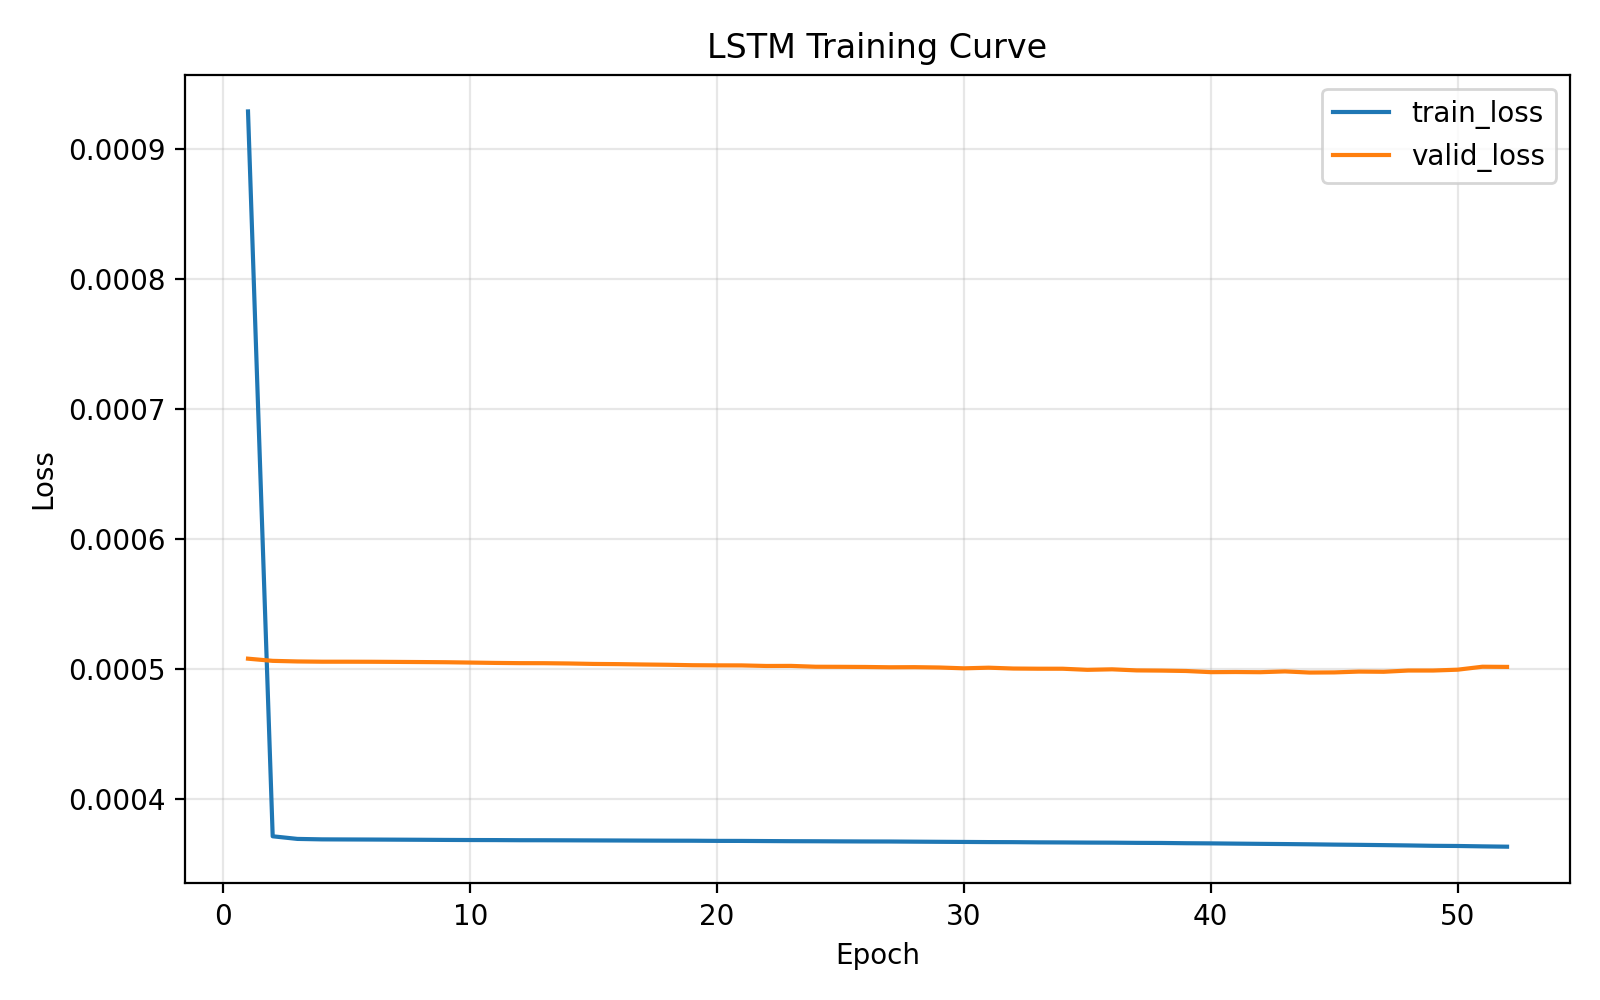
\includegraphics[width=0.72\linewidth]{outputs_lstm_seq10_oo_e60/figures/loss_curve_lstm.png}
\caption{LSTM seq10 严格 T+1 模型训练与验证损失曲线}\label{fig:loss}
\end{figure}

\section{策略与回测设计}

\subsection{预测指标}

基础预测指标包括日度 IC 均值、ICIR、RankIC、RankICIR 与方向胜率。
IC 衡量横截面预测分数与真实收益的线性相关性，RankIC 更关注排序关系；
ICIR 则用均值和日度波动的比值评价信号稳定性。

\subsection{交易策略}

回测从等权持仓出发，默认目标持仓数为 $n=10$，每日换仓参数为 $k=2$，均在作业建议区间内。
实现比较三类策略：
\begin{itemize}
  \item \textbf{Top10 Full：}每日直接持有预测分数最高的 10 只股票；
  \item \textbf{Top10-Drop2：}首日买入 Top10，之后仅卖出当前持仓中最低分的 2 只并补入高分股票；
  \item \textbf{Buffer-Risk：}使用排名缓冲区并加入短期涨跌幅、波动率与流动性近似过滤，限制频繁调仓。
\end{itemize}
此外对 Top10 策略运行随机分数基准，以检验模型信号是否优于随机选股。
严格 T+1 回测把信号日、买入日和卖出日显式分开：
\[
signal=t,\qquad buy=open(t+1),\qquad sell=open(t+2).
\]
净收益扣除按换手率近似的交易成本，默认费率为 0.0003。

\section{实验结果}

\subsection{标签口径对比}

两套标签在全样本上 Pearson 相关系数为 0.84468，Spearman 相关系数为 0.91707；
每日横截面 Spearman 均值也达到 0.90766。
这说明二者都刻画短周期收益排序，但并不等价。
$label_{\mathrm{oo}}$ 的标准差为 0.03238，高于 $label_{\mathrm{oc}}$ 的 0.02632，
反映出跨夜持有引入了额外波动。严格 T+1 报告应以 $label_{\mathrm{oo}}$ 为主，而不能只展示更乐观的日内估值收益。

\subsection{严格 T+1 主结果}

表~\ref{tab:oo-pred} 给出 2025 年严格 T+1 回测区间预测指标。LSTM seq10 在 ICIR 与 RankICIR 上稳定领先，
因此被选为比赛阶段主模型。

\begin{table}[H]
\centering
\caption{严格 T+1 真实执行预测指标}\label{tab:oo-pred}
\begin{tabular}{lrrrr}
\toprule
模型 & IC & ICIR & RankIC & DirectionAcc \\
\midrule
MLP & 0.04019 & 0.33985 & 0.03096 & 0.50497 \\
LSTM seq10 & 0.03581 & 0.42440 & 0.04112 & 0.51145 \\
LSTM seq20 & 0.02989 & 0.37405 & 0.03267 & 0.50371 \\
DLinear seq10 & 0.00868 & 0.12944 & 0.01622 & 0.49135 \\
DLinear seq20 & 0.01186 & 0.12960 & 0.02064 & 0.49131 \\
\bottomrule
\end{tabular}
\end{table}

\begin{table}[H]
\centering
\caption{LSTM seq10 严格 T+1 策略回测}\label{tab:lstm-oo-strategy}
\begin{tabular}{lrrrrr}
\toprule
策略 & 总收益 & 年化收益 & Sharpe & 最大回撤 & 平均换手 \\
\midrule
Top10 Full & 91.17\% & 102.15\% & 2.60 & -14.89\% & 1.5302 \\
Buffer-Risk & 54.79\% & 60.74\% & 1.97 & -14.53\% & 0.5983 \\
Top10-Drop2 & 43.71\% & 48.27\% & 1.62 & -16.58\% & 0.4026 \\
Random Top10-Drop2 & $27.63\%\pm14.48\%$ & $30.42\%\pm16.12\%$ & $1.23\pm0.49$ & -17.92\% & 0.4026 \\
Random Top10 Full & $12.10\%\pm12.20\%$ & $13.27\%\pm13.41\%$ & $0.63\pm0.52$ & -18.26\% & 1.9890 \\
\bottomrule
\end{tabular}
\end{table}

图~\ref{fig:t1-curves} 显示严格 T+1 回测中的净值与回撤。Top10 Full 收益最高，但平均换手超过 1.5；
Top10-Drop2 降低换手后仍优于对应随机基准，更适合在短期比赛里兼顾信号利用与执行成本。

\begin{figure}[H]
\centering
\begin{subfigure}{0.48\linewidth}
  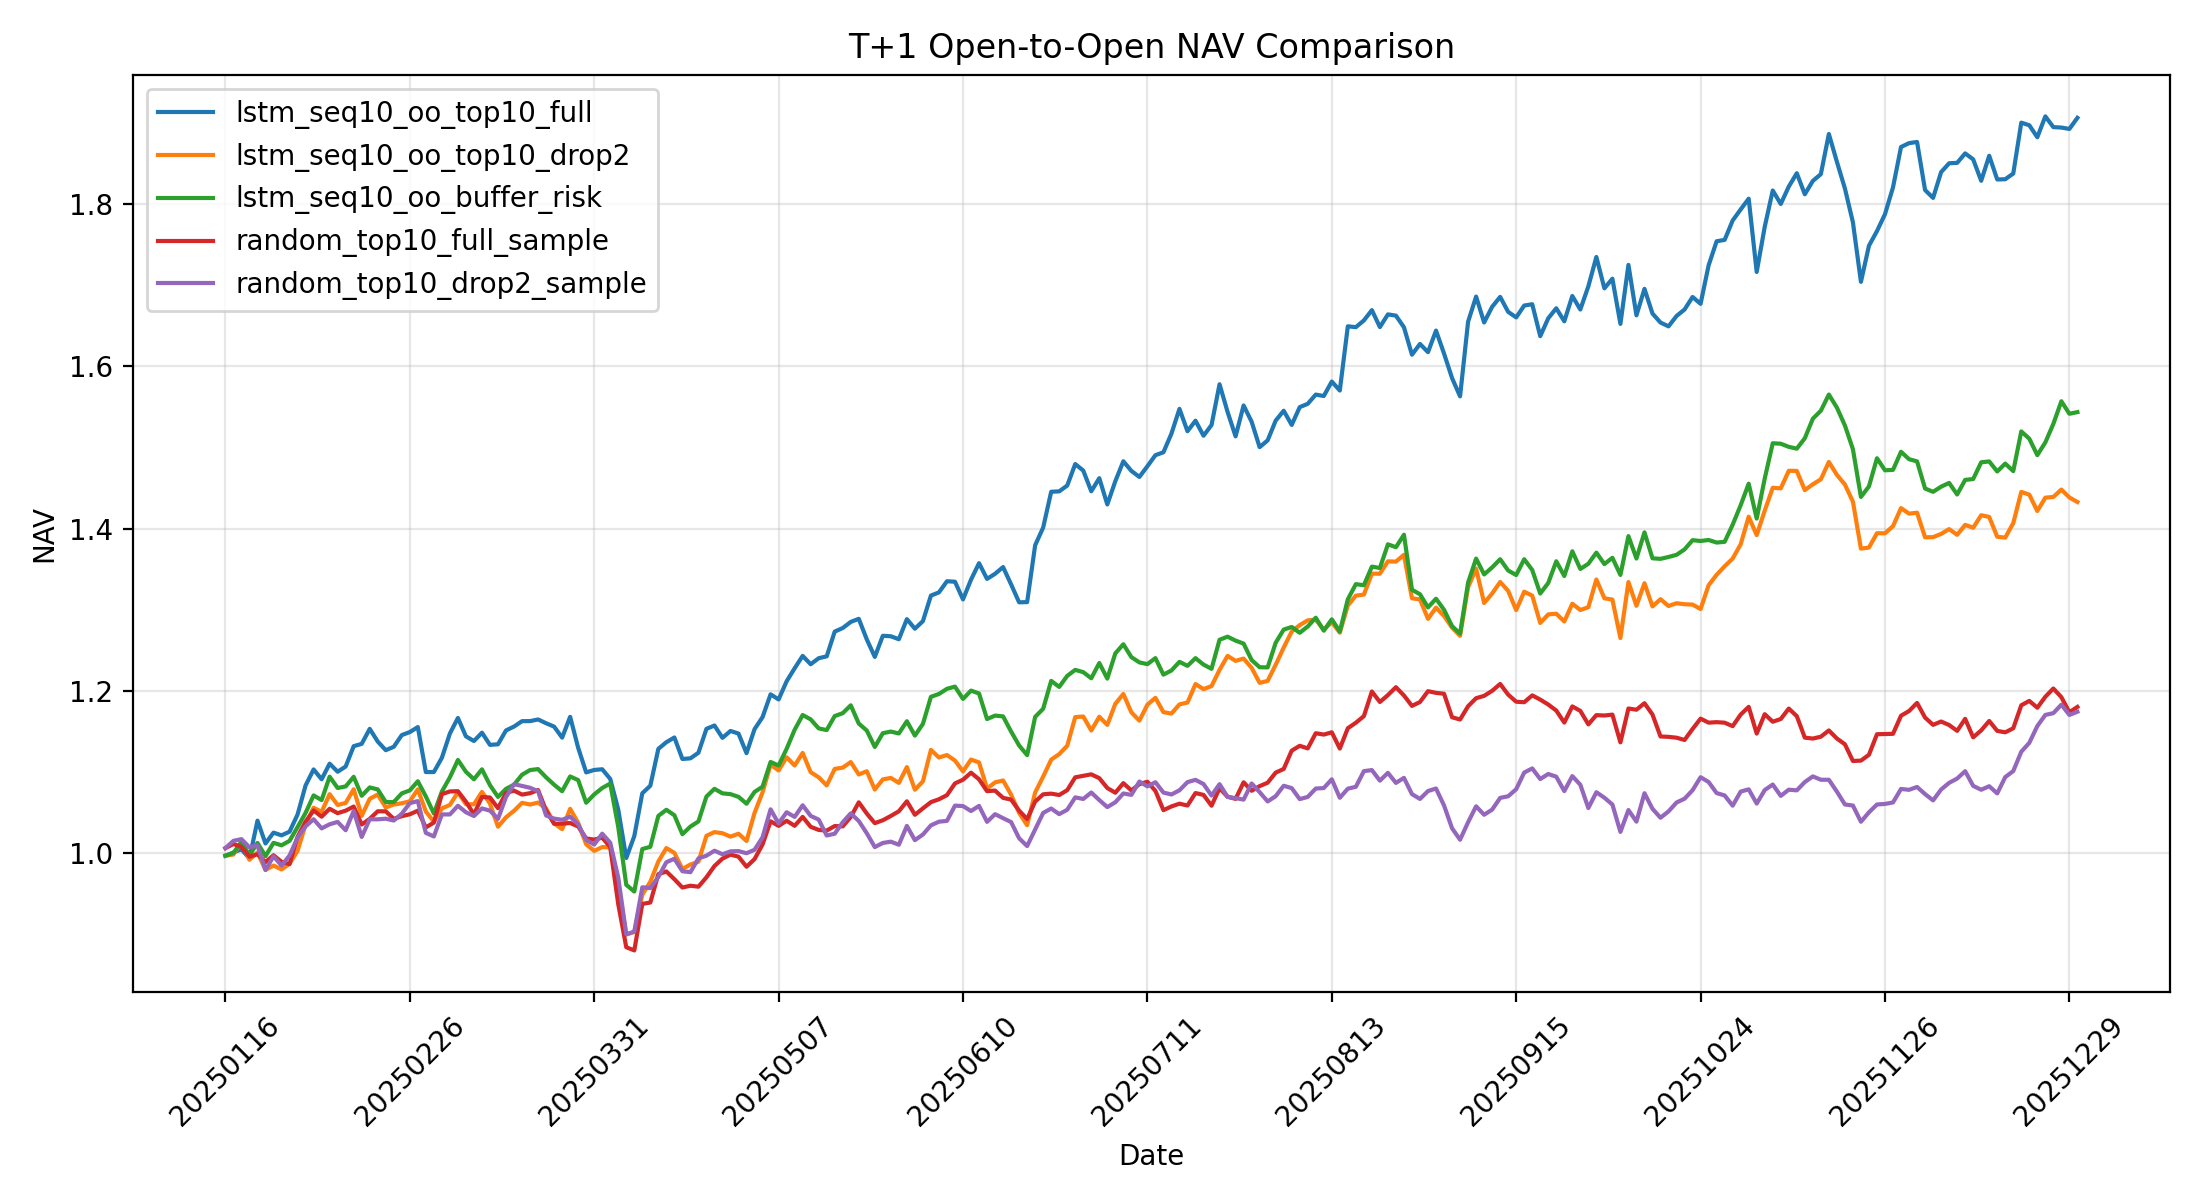
\includegraphics[width=\linewidth]{outputs_lstm_seq10_oo_e60/t1_backtest/strategy_nav_comparison_t1.png}
  \caption{策略净值}
\end{subfigure}
\hfill
\begin{subfigure}{0.48\linewidth}
  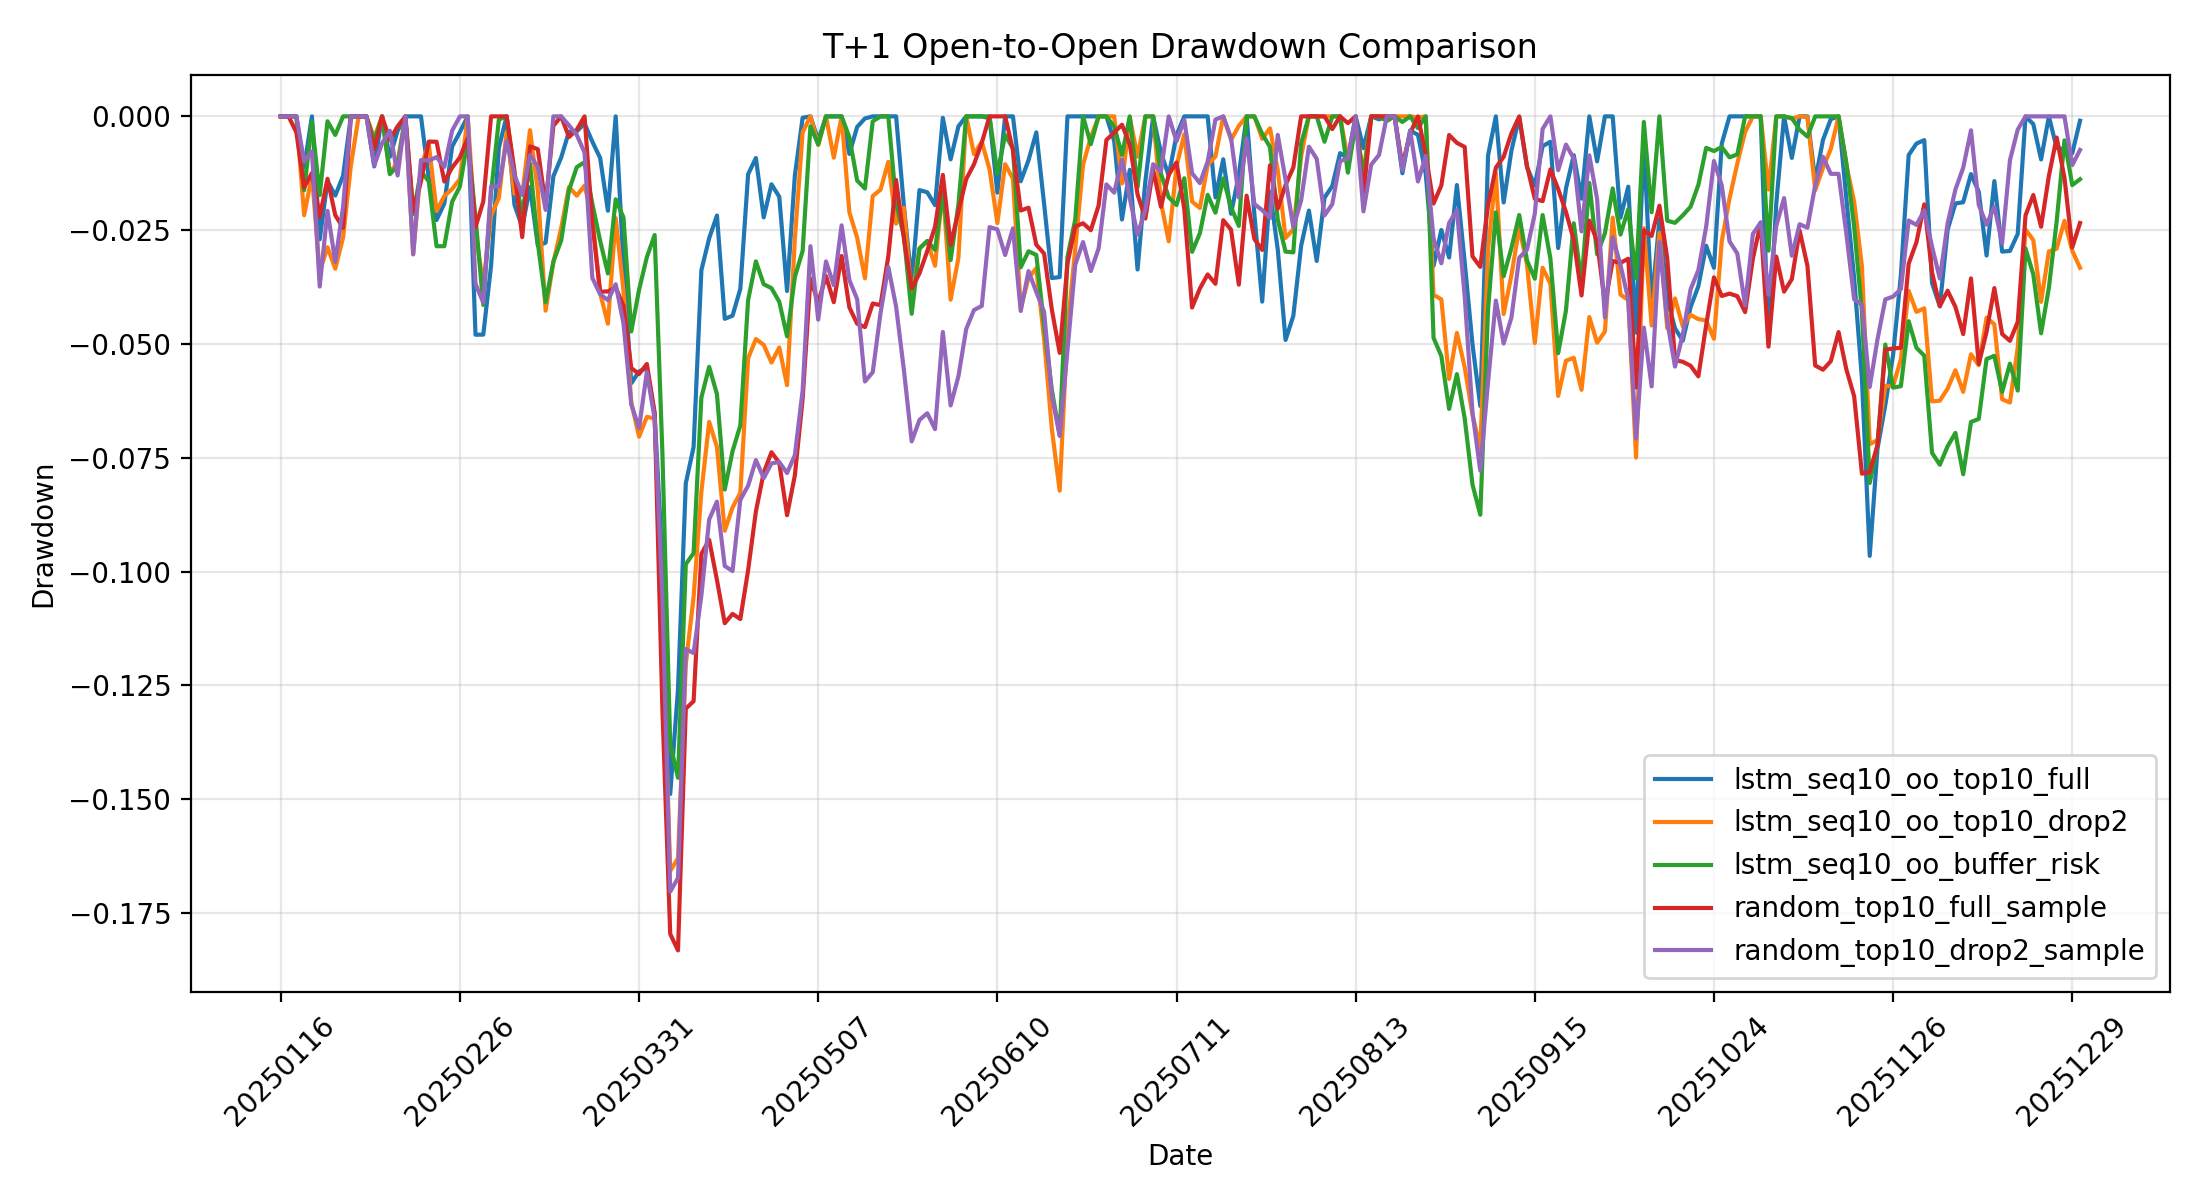
\includegraphics[width=\linewidth]{outputs_lstm_seq10_oo_e60/t1_backtest/strategy_drawdown_comparison_t1.png}
  \caption{策略回撤}
\end{subfigure}
\caption{LSTM seq10 严格 T+1 回测曲线}\label{fig:t1-curves}
\end{figure}

\subsection{OC 对照结果与模型比较}

$label_{\mathrm{oc}}$ 口径保留为研究对照。LSTM seq10 的 OC 回测 IC 为 0.02340、ICIR 为 0.26272；
Top10 Full 总收益为 183.77\%，Top10-Drop2 总收益为 172.62\%。
这些收益高于 OO 结果，但其收益定义包含买入当日收盘估值，因此不直接代表 T+1 可卖出的实现收益。
综合两套标签可见：MLP 是稳健的单日特征基线，LSTM seq10 能更好利用短历史窗口，
而 DLinear 在本任务上的信号和策略收益均较弱，适合作为线性序列对照而非最终交易模型。

\subsection{市场基准}

表~\ref{tab:index} 使用 2025 年主要指数基准做横向比较。
严格 T+1 的 LSTM seq10 Top10 Full 与 MLP Buffer-Risk 均高于三类指数；
低换手 LSTM seq10 Top10-Drop2 高于上证指数和沪深 300，但低于创业板指。

\begin{table}[H]
\centering
\caption{2025 年指数基准}\label{tab:index}
\begin{tabular}{lrrrr}
\toprule
指数 & 总收益 & 年化收益 & Sharpe & 最大回撤 \\
\midrule
上证指数 & 21.65\% & 22.53\% & 1.60 & -9.71\% \\
沪深 300 & 21.19\% & 22.06\% & 1.41 & -10.49\% \\
创业板指 & 55.46\% & 58.02\% & 1.72 & -20.79\% \\
\bottomrule
\end{tabular}
\end{table}

\subsection{交易成本敏感性}

短期横截面策略容易把预测优势换成高换手。表~\ref{tab:fee} 将费率从 0.0003 提高到 0.003。
Top10 Full 在高费率下快速退化，费率 0.003 时总收益转为 -26.44\%；
Top10-Drop2 因平均换手较低仍保留 12.00\% 总收益。
因此最终模拟交易默认采用 LSTM seq10 OO + Top10-Drop2，而不是只追求最低费率下的最高收益。

\begin{table}[H]
\centering
\caption{主策略交易成本敏感性}\label{tab:fee}
\begin{tabular}{llrrrr}
\toprule
策略 & Fee & 总收益 & 年化收益 & Sharpe & 平均换手 \\
\midrule
LSTM OO Top10 Full & 0.0003 & 91.17\% & 102.15\% & 2.60 & 1.5302 \\
LSTM OO Top10 Full & 0.0010 & 49.30\% & 54.54\% & 1.65 & 1.5302 \\
LSTM OO Top10 Full & 0.0030 & -26.44\% & -28.36\% & -1.05 & 1.5302 \\
LSTM OO Top10-Drop2 & 0.0003 & 43.71\% & 48.27\% & 1.62 & 0.4026 \\
LSTM OO Top10-Drop2 & 0.0010 & 34.72\% & 38.22\% & 1.35 & 0.4026 \\
LSTM OO Top10-Drop2 & 0.0030 & 12.00\% & 13.10\% & 0.58 & 0.4026 \\
\bottomrule
\end{tabular}
\end{table}

\section{实验亮点、局限与思考}

\subsection{实验亮点}

\begin{enumerate}
  \item 将日内估值标签与严格 T+1 open-to-open 标签分开，避免用不可直接落地的收益定义掩盖交易约束。
  \item 在模型之外比较策略、随机基准、指数基准和交易成本，使实验从预测指标延伸到实际执行质量。
  \item 使用同一特征体系对比 MLP、LSTM 和 DLinear，既保留课程神经网络主线，也能解释主模型选择。
  \item 增加每日预测脚本、交易计划脚本与 Streamlit 界面，能够用最新盘后数据生成比赛候选并维护真实持仓。
\end{enumerate}

\subsection{局限与反思}

历史回测仍是现实交易的近似。本文显式考虑手续费近似与 T+1 时间约束，但未完整建模涨跌停、停牌、最小成交单位和实际委托未成交。
此外，预测指标与最终收益并非单调关系：DLinear 的部分验证指标可为正，但策略表现仍弱；
Top10 Full 历史收益更高，却对成本更敏感。
这说明金融任务不能只根据单一 loss 或单一收益表选模型，还需要关注标签口径、排序稳定性、换手与执行可行性。

\section{模拟交易方案与赛后预留}\label{sec:simulation}

\subsection{比赛执行方案}

正式模拟交易期间默认采用 LSTM seq10 OO 主模型和 Top10-Drop2 策略。
每日在信号日盘后同步最新行情，复用训练期 checkpoint 与预处理状态生成候选分数；
交易日按计划先处理卖出，再补入高分股票，尽量维持满仓并遵守 T+1。
若 Streamlit 页面可用，则用页面维护 \texttt{data/current\_positions.csv}、生成买入/卖出/持有清单；
若页面不可用，则调用 \texttt{src/predict\_daily.py} 与 \texttt{src/make\_trade\_plan.py} 完成相同流程。

\subsection{赛后结果占位}

本节必须在比赛结束后补齐，提交前请不要删除该提醒。

\begin{table}[H]
\centering
\caption{模拟交易结果汇总占位表}
\begin{tabular}{p{0.34\linewidth}p{0.48\linewidth}}
\toprule
项目 & 赛后填写 \\
\midrule
比赛区间 & 2026-06-01 至 2026-06-12 \\
所用模型与策略 & LSTM seq10 OO + Top10-Drop2，若中途调整请说明原因 \\
初始资产与期末资产 & \todo{填入同花顺模拟盘结果} \\
区间收益率 & \todo{填入最终收益} \\
调仓次数与主要异常 & \todo{记录未成交、涨跌停、持仓偏离等情况} \\
与模型计划的一致性 & \todo{说明实际下单是否遵循每日候选与交易计划} \\
\bottomrule
\end{tabular}
\end{table}

\placeholderbox{4.2cm}{在此插入收益趋势截图\\建议文件：\texttt{report/figures/simulation\_equity.png}}
\placeholderbox{4.2cm}{在此插入调仓记录截图\\建议文件：\texttt{report/figures/simulation\_trades.png}}
\placeholderbox{4.2cm}{在此插入持仓记录截图\\建议文件：\texttt{report/figures/simulation\_positions.png}}

\subsection{赛后分析写作提示}

赛后分析建议回答三点：第一，真实收益与历史回测预期是否一致；第二，成交限制和满仓要求如何影响计划执行；
第三，短期比赛噪声下哪些经验可以反馈到标签、策略或风险控制设计。
这些内容直接对应作业中“收益记录、过程经验、感悟和思考”的评分要求。

\section{结论}

本文完成了课程要求的主体实验闭环：以课程 A 股量价数据为基础，构建可防泄露的时间切分和训练集预处理流程，
实现多种神经网络模型、历史回测、策略对照和每日交易辅助工具。
从严格 T+1 结果看，LSTM seq10 在预测稳定性和策略收益之间表现最好；
在考虑成本后，低换手 Top10-Drop2 是更适合模拟交易阶段的默认方案。
最终提交前仍需补齐组员信息、分工和正式比赛的真实截图与收益分析。

\appendix
\section{复现材料与输出文件}

代码仓库中与报告直接对应的主要文件如下：
\begin{itemize}
  \item 数据预处理：\texttt{src/data\_utils.py}；
  \item 模型定义：\texttt{src/model.py}, \texttt{src/model\_lstm.py}, \texttt{src/model\_dlinear.py}；
  \item 训练脚本：\texttt{src/train\_mlp.py}, \texttt{src/train\_lstm.py}, \texttt{src/train\_dlinear.py}；
  \item 严格 T+1 回测：\texttt{src/robust\_backtest\_t1\_all\_models.py}；
  \item 每日交易辅助：\texttt{src/predict\_daily.py}, \texttt{src/make\_trade\_plan.py}, \texttt{src/trading\_dashboard.py}；
  \item 主模型结果：\texttt{outputs\_lstm\_seq10\_oo\_e60/t1\_backtest/}；
  \item 指数与成本敏感性：\texttt{outputs\_benchmark/index/} 与 \texttt{outputs\_benchmark/fee\_sensitivity/}。
\end{itemize}

\section{提交前检查}

\begin{enumerate}
  \item 填写封面的两位组员姓名、学号和具体分工。
  \item 比赛结束后补入第~\ref{sec:simulation} 节的收益、调仓、持仓截图与文字分析。
  \item 保留 \texttt{requirements.txt}、\texttt{README.md}、全部源码和本报告源文件。
  \item 根据课程要求打包代码和报告；原始数据与模型权重可不随压缩包提交，但报告需说明数据来源。
\end{enumerate}

\end{document}
